\chapter{绪论}
\section{研究背景及意义}
\subsection{分布式深度学习的发展} \label{subsection_1_1_1}

在过去的几十年中，人工智能（AI）领域取得了显著的进展，对人们的日常生活和产业格局产生了深刻的影响。这一领域的迅速发展得益于多方面因素，包括计算机硬件性能的不断提升、海量的可用数据积累以及机器学习算法的不断改进。其中，深度学习作为机器学习的一个重要分支，在近几年逐渐崭露头角，引领了AI领域的创新浪潮。

%深度学习的兴起可以追溯到上世纪50年代，但在当时的计算资源限制下，深度神经网络的研究进展缓慢。然而，近年来，计算机性能的显著提升，尤其是图形处理单元（GPU）和专用硬件（如Google的Tensor Processing Unit，TPU）的出现，使得深度学习模型的训练和推理变得更加高效。此外，互联网的普及和数字化转型使得大量多样化的数据变得容易获取，这为深度学习提供了丰富的训练和测试资源。大数据的出现促使研究者更深入地探索神经网络的结构和参数，进一步推动了深度学习的发展。

深度学习因其卓越的特征提取能力以及多层神经网络在模拟人脑信息处理方式方面的杰出表现而著名\cite{fukushima1980neocognitron}。神经网络模型的高度非线性性质和其难以置信的大规模数据训练能力使其在众多领域中发挥着重要的作用。具体而言，在计算机视觉领域，卷积神经网络（CNN）\cite{szegedy2015going, simonyan2014very, he2016deep, ren2015faster}已经在图像分类、物体检测和图像生成等任务中取得卓越成绩。在自然语言处理领域，循环神经网络（RNN）\cite{bahdanau2014neural, graves2013generating, socher2013recursive}和变换器（Transformer）\cite{vaswani2017attention, devlin2018bert}等模型使得机器翻译、文本生成和情感分析等任务取得重大进展。此外，深度强化学习在游戏领域和机器人控制等领域表现出了强大的学习能力\cite{mnih2013playing, lillicrap2015continuous, haarnoja2018soft}。特别值得关注的是，OpenAI公司最近研发的智能聊天机器人ChatGPT，在自然语言处理领域取得了显著的突破。ChatGPT具有卓越的自然语言理解和生成能力\cite{liu2023summary}，能够深入理解和学习用户的语言模式，从而协助用户完成诗歌创作、邮件撰写以及内容检索等各种任务。ChatGPT的出现代表了深度学习在处理复杂自然语言任务方面的巨大进步，为改善人机交互、自动化客户服务、教育辅助等领域提供了创新性的解决方案。由此可见，深度学习的兴起已经很大程度上改变了AI研究和应用的方式，使其能够解决以前被认为不可能的复杂问题。

鉴于深度学习在各个领域的突出表现，对于深度学习及其相关的交叉领域的研究热度逐年提升。
%图是2010年以来全球发表深度学习相关论文数量的变化情况，可以看到，在深度学习的发展初期，发表论文数呈现指数级别增长，截至2022年底相关论文已经发表数十万篇。
% 2010 79；2011 103； 2012 153；2013 295；2014 738；2015 1810；2016 3833；2017 9423；2018 20953；2019 31389；2020 50792；2021 72626；2022 76111
%\textcolor{red}{此处插入一个近十年全球深度学习论文发表数变化的图片（数据来源：Web of Science）}
%随着深度学习领域研究的不断深入，
为了在实际应用中取得更好的训练效果，一方面，深度学习所使用的数据集越来越大。例如，计算机视觉领域常用的ImageNet数据集\cite{deng2009imagenet}包含约128万张图片，总大小超过150GB；面向其他采用高分辨率图像或视频的领域的数据集甚至高达TB乃至PB级别。另一方面，深度学习使用的网络模型规模急剧增加，例如Google公司提出的Switch-C模型\cite{fedus2022switch}具有16000亿参数，Meta（Facebook）公司提出的大语音模型OPT-175B\cite{zhang2022opt}，以及OpenAI提出GPT-3\cite{brown2020language}都具有超1750亿参数。\autoref{fig:Fig1-1}展示了近年来大规模深度神经网络模型的发展。

\captionsetup[figure]{labelformat=simple, labelsep=space}
\begin{figure}[!htbp]
    \centering
    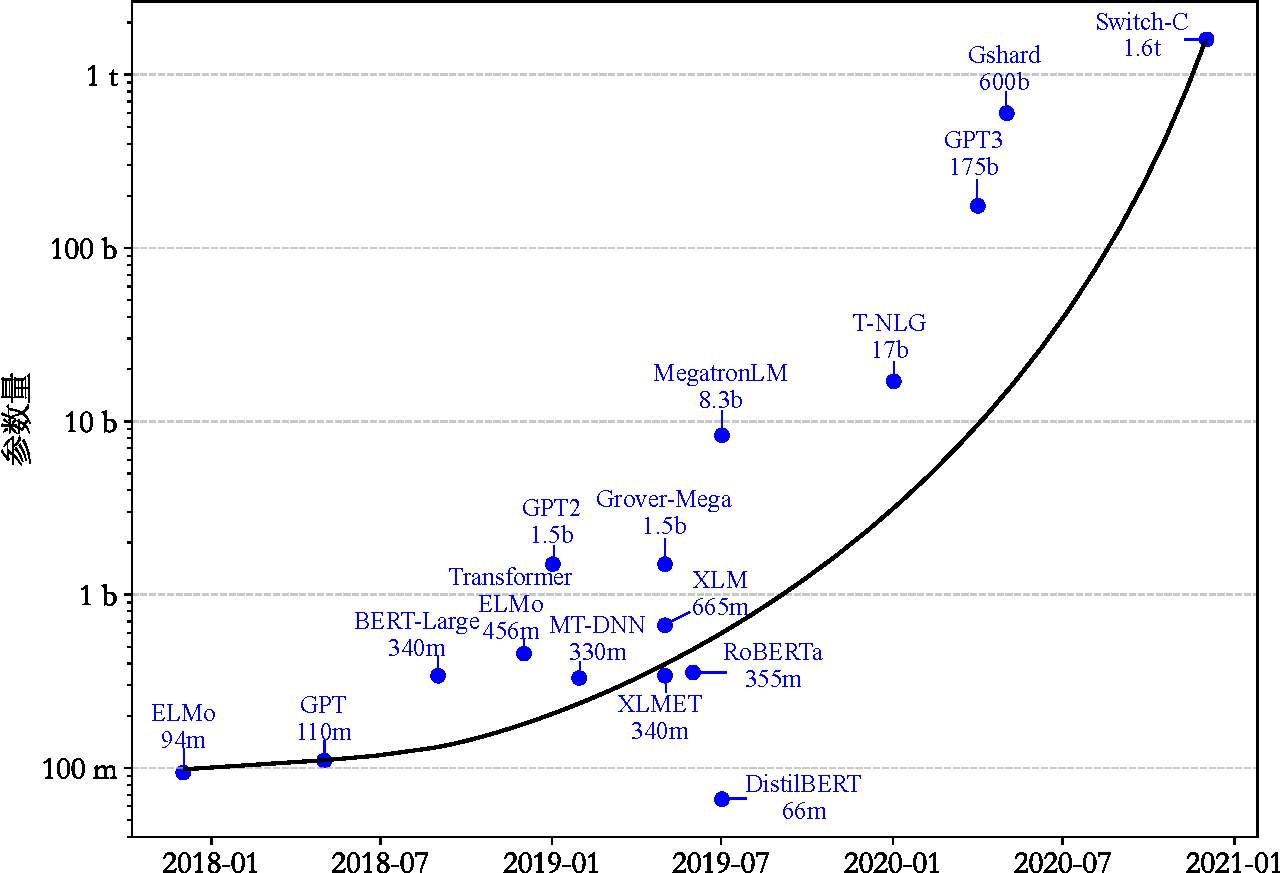
\includegraphics[width=5in]{figure/chapter1/fig1-1-nn_params.pdf}
    \caption{\label{fig:Fig1-1}大规模深度神经网络模型的发展情况（数据来源：OpenAI）}
\end{figure}

数据和模型规模的增大使得深度学习应用所需的算力越来越大，这促使了GPU等加速器设备的研究不断发展。以Nvidia GPU发展为例，\autoref{tab:GPU性能}展示了2012年以来Nvidia的多代GPU在训练ResNet模型时的性能表现。从表中可以发现，2012年至2019年的8年时间，GPU的计算能力仅提高了16倍左右，而同时期的深度神经网络模型的训练所需要的算力呈指数级别增长，这使得单个GPU的性能逐渐无法满足深度学习任务的需求。除此之外，大规模的数据集和深度神经网络模型需要大量的内存空间，单个设备也逐渐无法存放训练所需的完整的数据集和模型。因此，面对日益复杂的深度学习任务，分布式深度学习被认为是必然的发展趋势，逐渐成为业界的研究热点\cite{ben2019demystifying}。

%统一版本，调整表格整体长度到适合自己的大小为止，
\begin{table}[!htbp]
    \centering
    \caption{单GPU训练ResNet-269模型的性能\cite{luo2018parameter}}
    \label{tab:GPU性能}
    \setlength{\tabcolsep}{5mm}{%可随机设置，调整表格整体长度到适合自己的大小为止
            \begin{tabular}{ccc}
                \toprule[2pt]
            \multicolumn{1}{l}{GPU型号} & \multicolumn{1}{l}{发布时间} & \multicolumn{1}{l}{训练速度（图片/秒）} \\ \midrule[1pt]
            K520                     & 2012年 &4     \\
            K80                  & 2014年 &11        \\
            M60                     &2015年 & 14  \\
            1080Ti                   & 2017年 & 44\\ 
            V100                   &2019年& 65     \\\bottomrule[2pt]
            
            \end{tabular}
    }
\end{table}

分布式深度学习将训练任务拆分到多个计算节点（即GPU设备），每个节点在迭代过程中依次执行本地计算任务和与其他节点的通信任务，从而协同完成全局目标的优化。通常情况下，对于一个由$n$个节点构成的大规模深度学习任务，其分布式深度学习模型可以描述成如下的优化问题\cite{smola2010architecture}：
\begin{equation}
    \label{equ:distributed_training_optimization_object}
    \min_x \!\:F\left( x \right) \coloneqq \frac{1}{n}\sum_{i=1}^n{\underset{=:f_i(x)}{\underbrace{\mathbb{E}_{\xi _i\sim D_i}l(x;\xi _i)}}}
\end{equation}
其中$x\in \mathbb{R}^d$是模型参数，$D_i$是节点$i$的本地数据集，$\xi _i$是节点$i$的本地数据集中的样本，$l\left( \cdot \right) $是样本的损失函数，$f_i\left( \cdot \right) $是节点$i$本地所有数据样本的损失函数的平均值，$F\left( \cdot \right)$是所有节点损失函数的平均值。该模型训练的最终目标是找到最优的$x^*$，从而使得损失函数的平均值最小。

分布式深度学习主要采用数据并行和模型并行的方式进行深度神经网络模型的训练\cite{tang2020communication}。如\autoref{fig:Fig1-2}所示，在数据并行的训练方式中，首先，数据集被根据一定的划分策略分配到不同的计算节点（即GPU设备）上，然后每个计算节点利用本地数据集训练相同的深度神经网络模型，并且在训练的每次迭代中进行模型梯度或者模型参数的通信，从而实现在若干次迭代后每个节点的模型参数能够收敛到一致的全局最优解。在模型并行的训练方式中，神经网络模型被划分到不同的计算节点上，并且在每次迭代过程中，每个节点首先等待接收其前一个神经网络层所在节点的输出，然后完成本地子模型的训练并将本地子模型的输出发送给下一个节点，从而完成整个深度神经网络模型的训练。其模型划分方式包括水平拆分、垂直拆分和混合拆分\cite{tang2020communication}。数据并行由于实现起来较为简单，并且不同节点的计算负载比较均衡，应用最为广泛。目前大多数主流的深度学习框架都对数据并行提供了支持，并且具有很好的易用性，而模型并行仍需要用户手动对模型进行划分和分布式部署，因此本文将围绕数据并行展开研究。

\begin{figure}[!htbp]
    \centering
    \subfigure[数据并行训练方式]{
        % \fbox{
        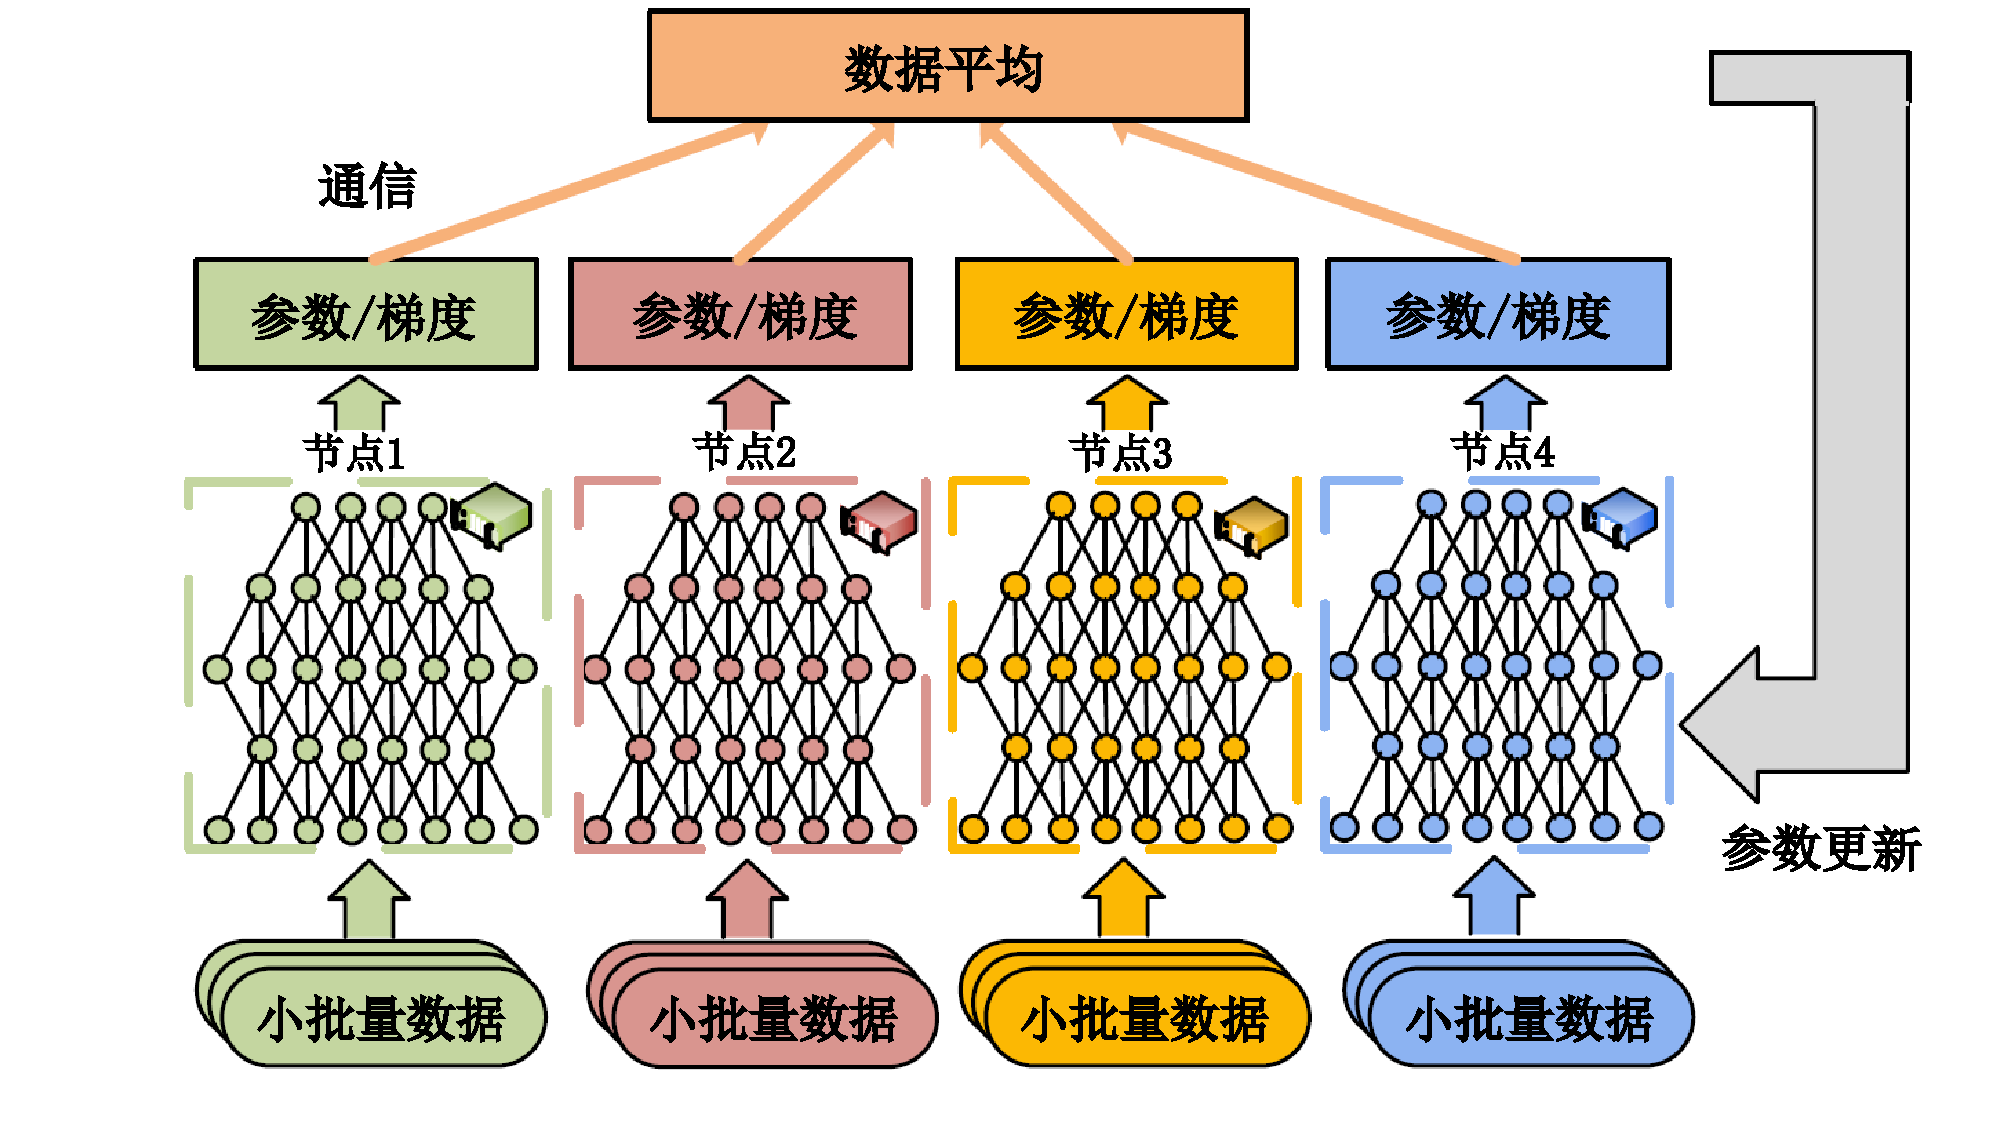
\includegraphics[width=0.5\linewidth]{figure/chapter1/fig1-2-data_parallel.pdf}
        % }
        \label{fig:Fig1-2-data-parallel}%文中引用该图片代号
    }
    \subfigure[模型并行训练方式]{
        % \fbox{
        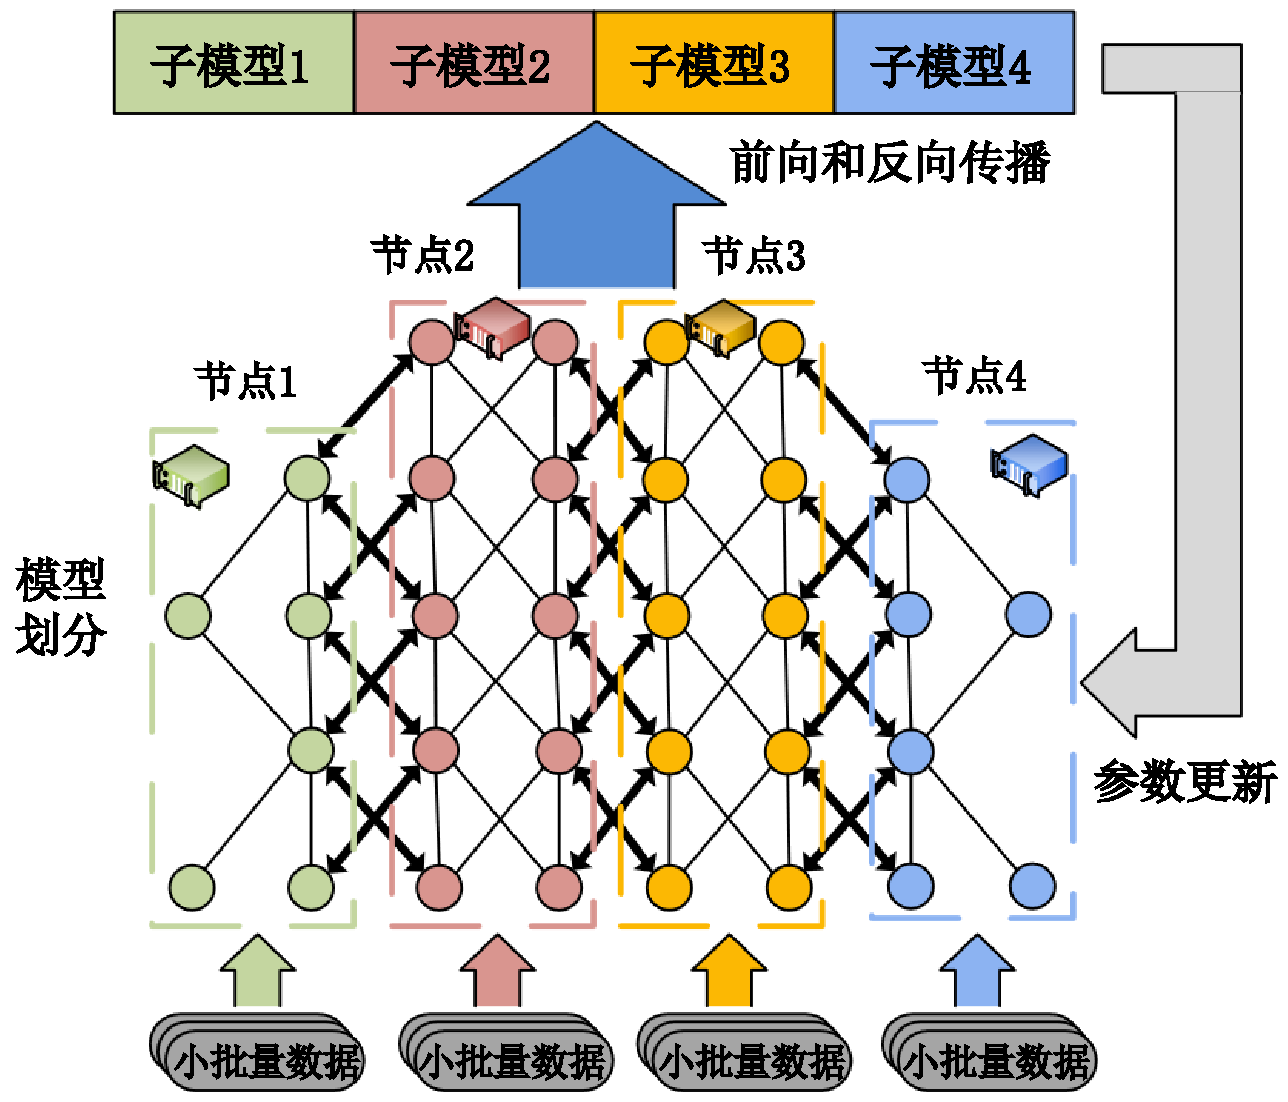
\includegraphics[width=0.4\linewidth]{figure/chapter1/fig1-2-model_parallel.pdf}
        % }
        \label{fig:Fig1-2-model-parallel}%文中引用该图片代号
    }
    \caption{分布式深度学习并行训练方式}
    \label{fig:Fig1-2}
\end{figure}

分布式深度学习的训练技术发展至今天已经十分成熟，衍生出了各种训练架构和算法。如图所示，分布式训练中常用的三种架构包括参数服务器（Parameter Server，简称PS）架构\cite{li2014communication}、全归约（All-Reduce）架构\cite{sergeev2018horovod}以及去中心化的分布式（Gossip）架构\cite{kempe2003gossip, lian2017can}。PS架构将计算节点分为参数服务器组和工作者组，参数服务器组负责汇总工作者组的参数/梯度，计算平均值并用于更新全局模型参数，工作者组则在每次迭代中依次执行从参数服务器组拉取模型参数、利用本地数据集训练模型和将最新的模型参数/梯度推送给参数服务器组。在该架构中，参数服务器节点是拓扑的中心，因此也通常被称为集中式架构。All-Reduce架构则是一种典型的无中心的训练架构，在该架构中每个节点都需要汇总其他节点的参数/梯度。为了实现该通信机制，需要在给定的拓扑上采用一定的通信策略将每个节点的数据发送给其他所有节点。根据PS架构和All-Reduce架构的训练特点，这两类架构都能够保证每次迭代中模型参数的一致性。与之不同，Gossip架构采用完全分布式的拓扑结构，其中每个计算节点只与拓扑中相连的计算节点进行通信，因此相比于前两种架构更加灵活，但是需要选择合适的拓扑结构和训练算法来保证不同节点的模型参数最终能够收敛到一致。基于这些架构，国内外的学者提出了许多分布式优化算法用于机器学习和深度学习的训练中，根据计算和通信的时序性，这些算法可以分为同步算法\cite{mcmahan2017communication, goyal2017accurate, lian2017can, tang2018d, zhang2019decentralized, xin2019distributed}和异步算法\cite{recht2011hogwild, agarwal2011distributed, lian2018asynchronous, lian2015asynchronous, zhang2015staleness, zhou2022towards}，其中同步算法要求各节点的计算和通信同步进行，因此容易受到慢节点的影响，而异步算法更加灵活，各节点的计算和通信相对独立，考虑了设备之间的计算异构性以及通信延时。本文的研究将聚焦于All-Reduce架构和Gossip架构以及基于这两种架构的同步算法。

\begin{figure}[!htbp]
    \centering
    \subfigure[PS架构]{
        % \fbox{
        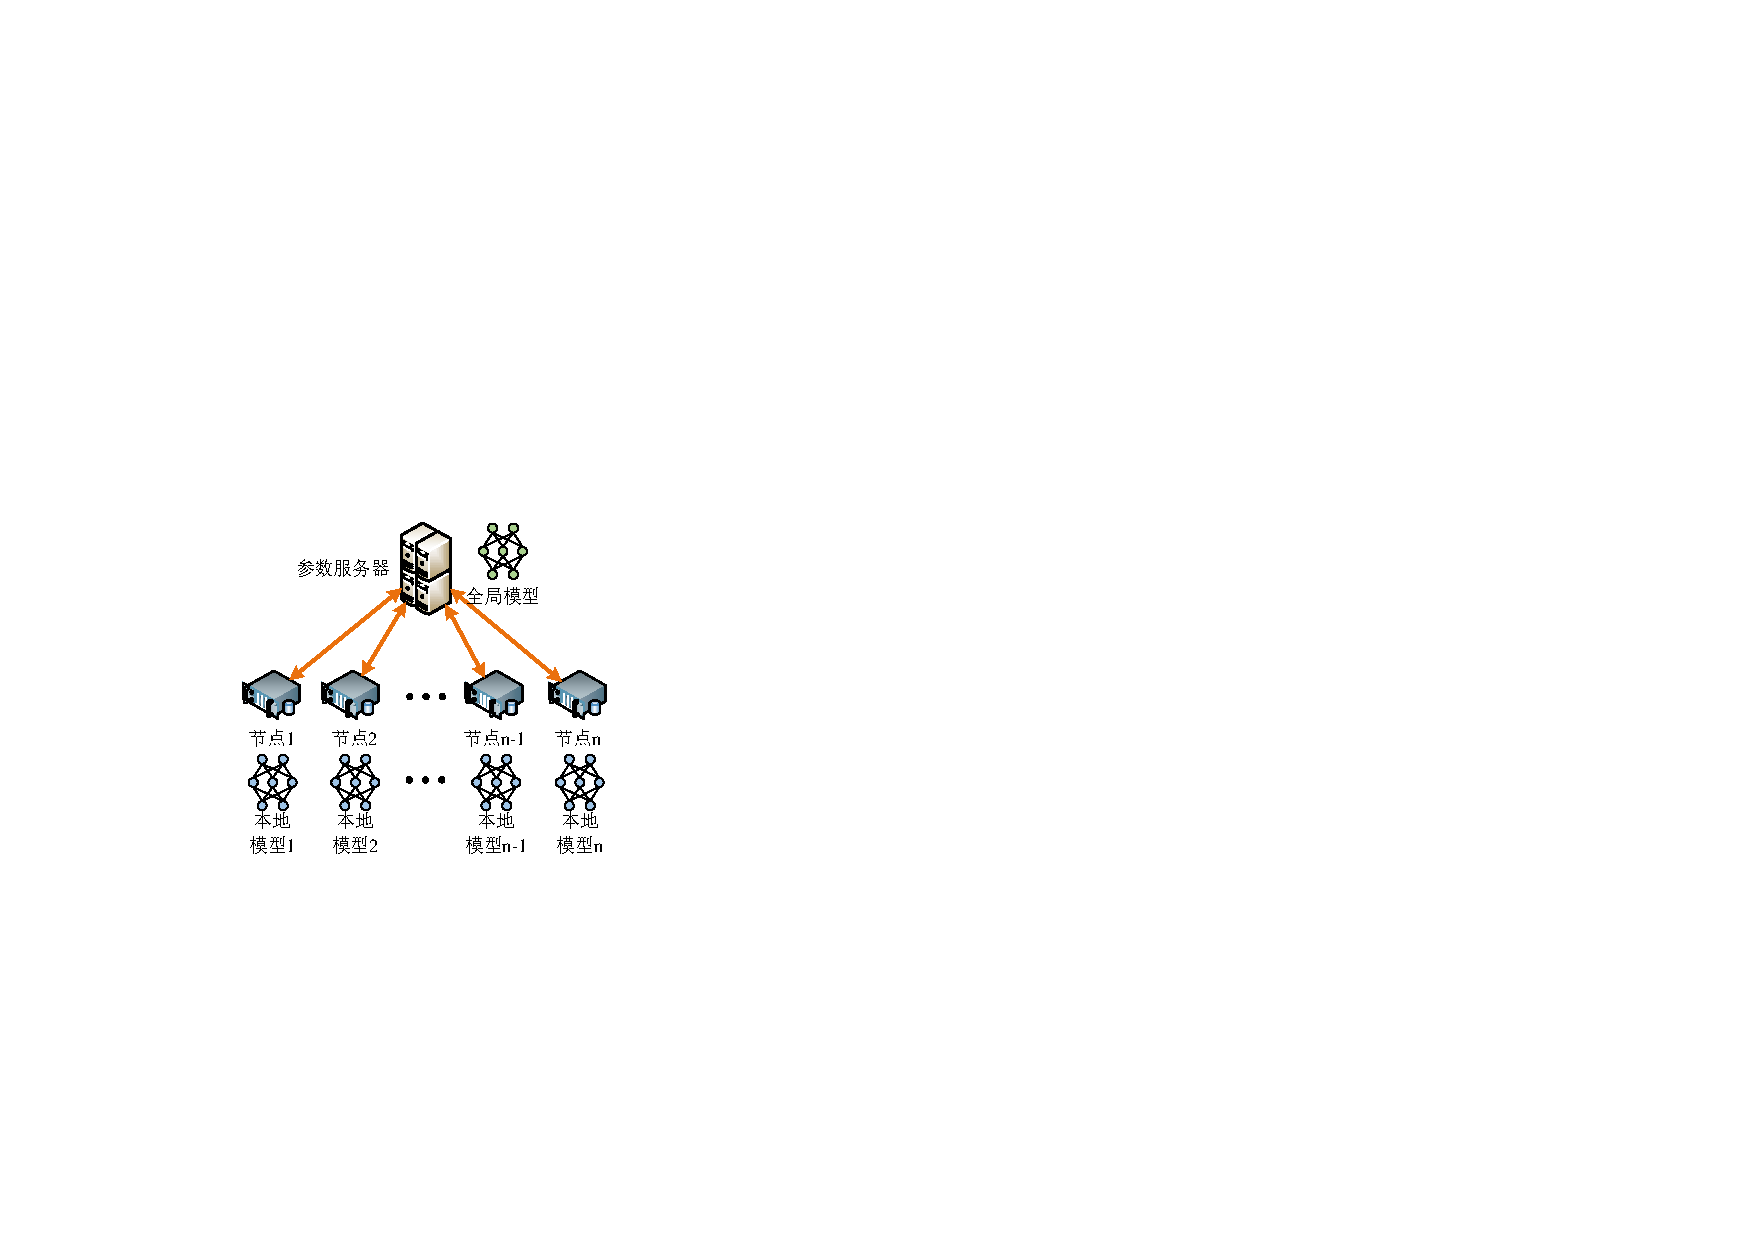
\includegraphics[width=0.3\linewidth]{figure/chapter1/fig1-3-PS.pdf}
        % }
        \label{fig:Fig1-3-PS}%文中引用该图片代号
    }
    \subfigure[All-Reduce架构]{
        % \fbox{
        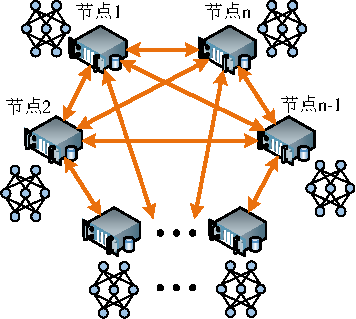
\includegraphics[width=0.3\linewidth]{figure/chapter1/fig1-3-2-AllReduce.pdf}
        % }
        \label{fig:Fig1-3-allreduce}%文中引用该图片代号
    }
    \subfigure[Gossip架构]{
        % \fbox{
        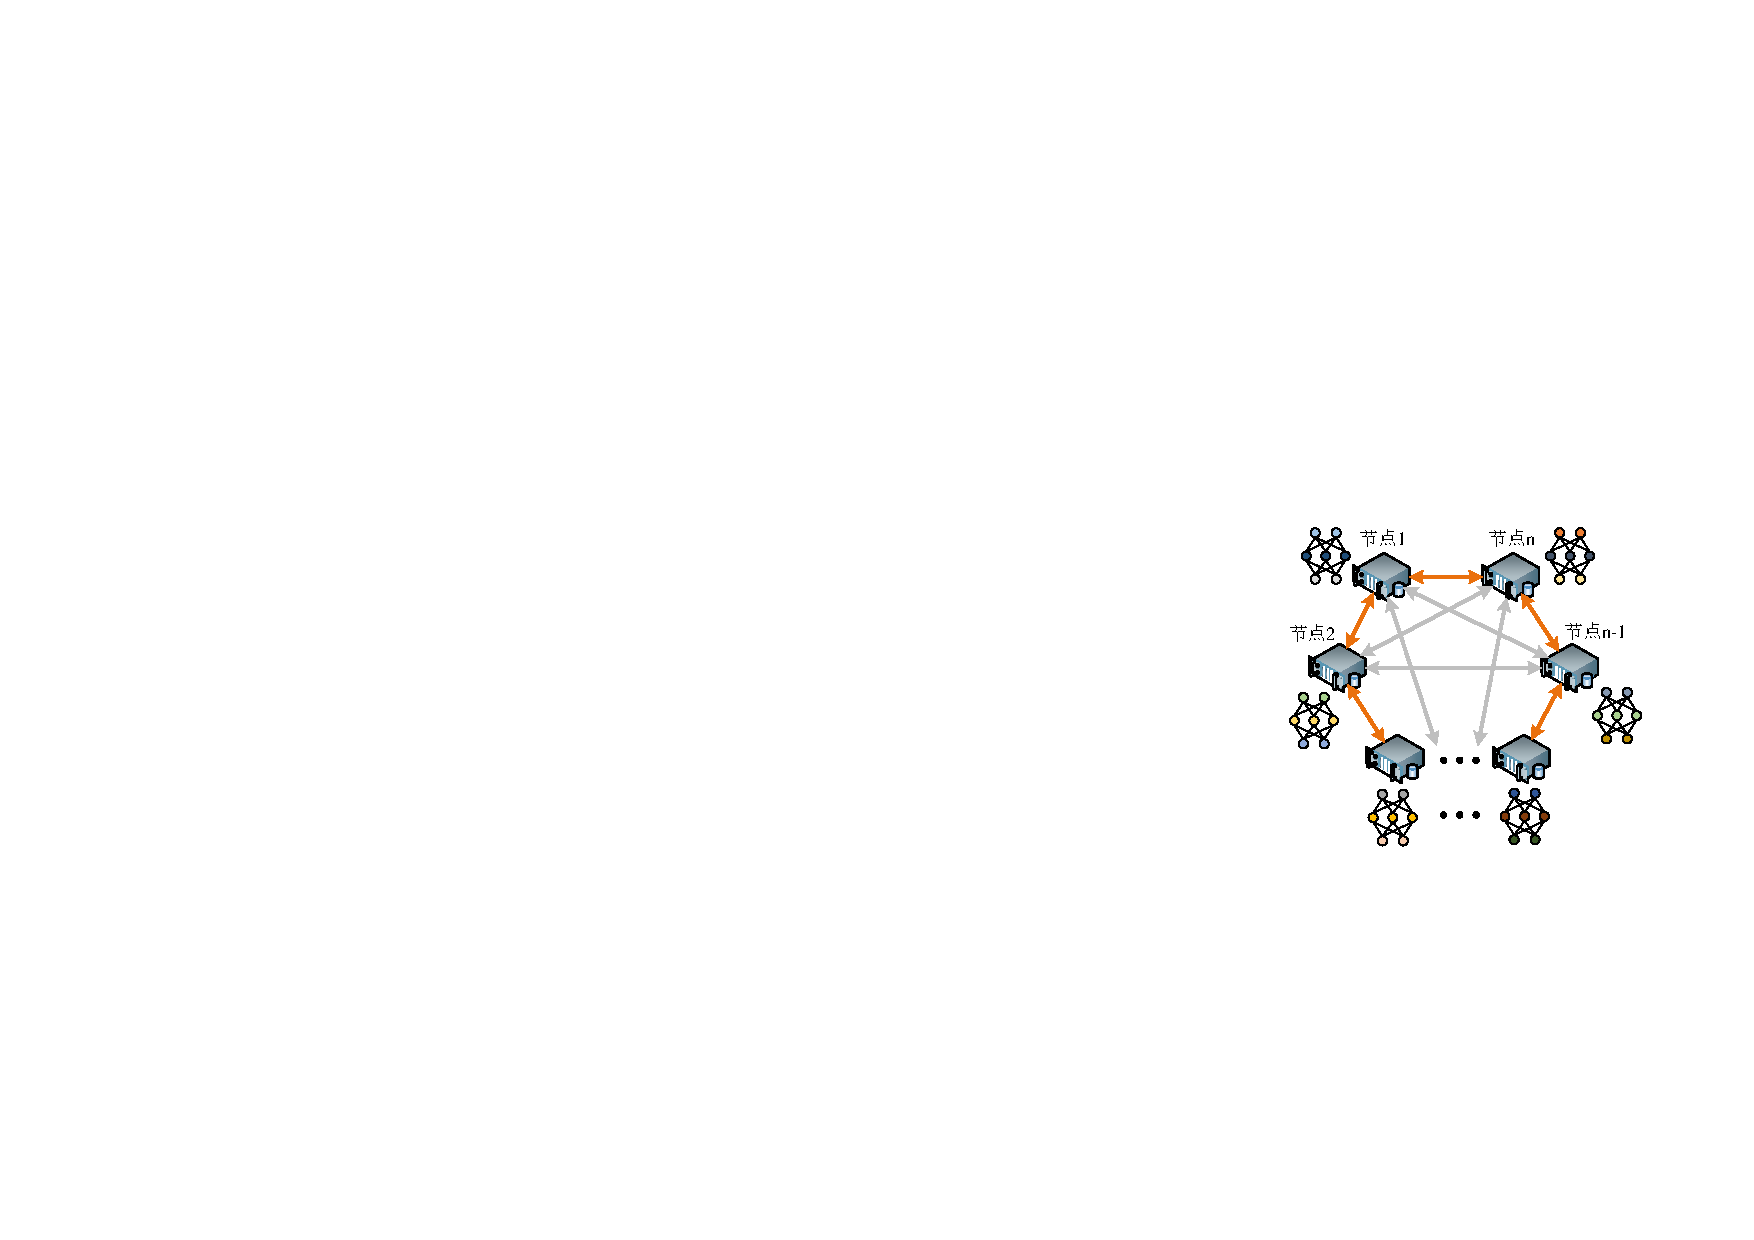
\includegraphics[width=0.3\linewidth]{figure/chapter1/fig1-3-3-Gossip.pdf}
        % }
        \label{fig:Fig1-3-gossip}%文中引用该图片代号
    }
    \caption{分布式深度学习训练架构}
    \label{fig:Fig1-3}
\end{figure}


随着现实场景中深度学习任务的复杂性不断提高，训练深度神经网络模型所需的计算和通信资源越来越多，因此分布式深度学习的性能（如训练时间、功耗等）逐渐引起研究人员们的关注。在保证模型精度的前提下提高分布式训练的性能，从而节约训练资源，对分布式深度学习技术的可持续发展有着重要的意义。%本文主要围绕训练时间这一性能展开研究。

\subsection{基于通信优化的分布式训练加速的必要性}

分布式深度学习的主要目标就是加快深度学习任务的训练速度，因此加速比常被用来衡量分布式深度学习的加速效果\cite{王帅2022}，即同一深度学习训练任务在单机训练和分布式训练时所需时间的比值。理想情况下，加速比随着节点数目线性增加，而由于节点间通信的存在，这一线性关系很难实现。现实场景中加速比随节点数目的变化趋势为先升高后降低，即在一定的规模内，随着节点数目的增加，加速比逐渐增加，当节点数目超过一定规模时，加速比将不再增加，并且会逐渐减小，这是因为通信开销抵消了节点增加所带来的计算性能上的增益，从而导致资源的浪费。鉴于分布式训练性能变化的特点，对于大规模的分布式深度学习任务，分析可能的性能瓶颈，从而合理地配置集群规模，对于加快分布式训练速度和避免计算资源的浪费具有重要意义。

然而，大规模分布式深度学习任务的训练通常需要花费很长时间，无论训练是在云上还是在本地提供的资源上执行，这都将导致过高的训练成本。因此，预测分布式训练所需时间成为一种有效的解决方案，可以帮助我们在较短的时间里评估不同集群规模上分布式深度学习任务所需的训练时间，从而在实际部署神经网络模型之前确定合适的集群规模，节约昂贵的计算资源和时间成本。另外，通过训练时间预测可以得到分布式训练过程中各部分的执行时间，从而为训练时间的优化提供帮助。

如前文所述，加速比的减小主要由节点之间的通信导致。具体来讲，在分布式深度学习中，由于每个计算节点本地只有部分训练数据或模型，为了保证最终得到的模型与单机上利用完整数据集训练的模型一致，计算节点之间需要频繁地进行数据的通信，以同步模型参数。随着节点数目的增加，一方面，集群中通信次数逐渐增加，使得通信开销变大；另一方面，每个计算节点分配的数据集或模型规模逐渐减小，相应的计算开销变小。因此，随着分布式深度学习系统规模的不断增大，通信开销在整体训练开销中的占比逐渐变大，节点的等待时间变长，整体训练效率降低。因此研究通信性能的优化对于改善分布式深度学习系统的网络性能、提高分布式训练的效率具有重要的意义。

影响分布式深度学习通信性能的重要因素之一是集群的通信拓扑\cite{neglia2019role, wang2021impact, nedic2018network}，本文将其称为参数同步拓扑。该拓扑决定了迭代过程中每个计算节点与哪些邻居节点进行通信，从而决定了每次迭代的通信开销。此外，拓扑的连通性以及参数同步的权重矩阵决定了一致性的速度，进而影响着迭代复杂度，即神经网络模型收敛所需的迭代次数，所以参数同步拓扑间接影响着分布式深度学习的总通信次数。因此，参数同步拓扑对整体训练时间起着至关重要的作用，研究参数同步拓扑的优化可以帮助提高分布式训练的通信效率，加快模型的收敛速度，从而缩短训练时间。影响通信时间的另一重要因素是节点之间通信的数据量。近年来，神经网络模型规模越来越大，模型参数量不断增加，节点之间通信的数据量也随之增加，从而加剧了分布式训练的网络通信压力。由于通信数据量对通信时间的影响往往是线性的，所以在不丢失数据中关键信息的前提下压缩通信的数据可以很大程度上缩短通信时间。

综上所述，本文将首先研究分布式深度学习的训练时间预测技术，实现对分布式深度学习训练时间的准确预测，从而帮助分析性能瓶颈，然后分别从参数同步拓扑和通信数据量出发，对分布式深度学习的通信时间进行优化，以尽可能缩短训练时间。


\subsection{基于通信优化的分布式训练加速的研究挑战}

在分布式深度学习中，训练时间直接影响到资源的利用率和开销，包括计算资源、存储资源和网络带宽，而大规模深度神经网络模型的训练任务往往需要在GPU集群上花费较长时间完成，因此分布式深度学习的训练时间预测与优化技术对于节约训练成本十分关键。根据分布式深度学习的特点，其训练时间预测与优化的难点与挑战主要有以下三点：

\begin{itemize}
    \item [（1）] 建立准确的训练时间预测模型难。影响分布式深度学习训练时间的特征众多，这些特征之间依赖性强，并且特征与训练时间之间呈现复杂的非线性关系，此外，分布式深度学习的计算与通信之间存在一定的耦合关系，难以建立准确的训练时间预测模型。
    \item [（2）] 设计高效的参数同步拓扑难。在分布式深度学习中，参数同步拓扑对每次迭代所需的通信开销和迭代复杂度的作用往往相反，即稀疏的拓扑每次迭代所需的通信开销小而迭代复杂度高，反之同理，难以权衡二者设计高效的参数同步拓扑。
    \item [（3）] 高精度的通信数据压缩难。数据的压缩往往会带来信息的丢失，由于分布式深度学习中通信的数据往往是神经网络模型的参数或者梯度，对其进行压缩会不仅导致模型的收敛速度变慢，而且会导致模型精度下降，难以在保证模型精度的前提下对通信的数据进行高效地压缩。
\end{itemize}

综上所述，研究分布式深度学习的训练时间预测与优化技术具有重要意义。通过建立准确的分布式深度学习训练时间预测模型、设计高效的参数同步拓扑和通信数据压缩策略，可以提高分布式训练的速度，节约训练资源，从而实现分布式深度学习技术的可持续发展。%这将为高效、可扩展的深度学习训练框架和系统的实现，以及深度学习在各个领域的广泛应用，提供重要的理论和实践基础。

\section{国内外研究现状}

随着分布式深度学习系统规模的增大，分布式训练的性能逐渐引起研究人员们的关注，其中训练时间作为性能度量的重要指标之一，对其进行预测和优化可以帮助研究人员和工程师更好地规划资源，从而提高分布式深度学习的训练效率，节约训练资源。本文将面向分布式深度学习的训练时间预测与优化技术研究大致分为三个部分，分别是训练时间预测技术、参数同步拓扑结构优化技术和通信数据压缩技术。以下将详细介绍这三个研究内容的国内外研究现状。

\subsection{集合通信算法设计}

分布式训练中常用的集合通信算子有AllReduce、ReduceScatter、AllGather、AlltoAll等，其中AllReduce是最常用的算子，AllReduce算子将所有节点的数据进行规约（如求和、求平均等），并将结果分发到所有节点上。在分布式训练中，AllReduce通常用于同步各节点的模型参数或梯度，从而保证每个节点在每次迭代后都拥有一致的模型参数。AllReduce可以看作是ReduceScatter和AllGather两个算子的组合，首先通过ReduceScatter将所有节点的数据进行规约并分发到各节点上，然后通过AllGather将规约后的结果汇总到所有节点上。AllReduce的大部分算法实现也可以拆分成ReduceScatter和AllGather两部分，因此大部分经典研究都是针对AllReduce算子的。除此之外，随着大模型架构的发展，AlltoAll开始广泛应用于分布式训练场景中，如模型并行训练中不同节点间的特征交换和混合专家模型（Mixture of Experts，MOE）中的dispatch和combine操作等。

集合通信算子的具体实现与性能表现都和硬件平台密切相关，为了方便不同硬件环境下的集合通信算子的高效实现，业界将与底层硬件和通信协议相关的实现封装起来，提供了多种集合通信库作为集合通算子的实现接口以及开发平台。对于集合通信算子的具体实现算法，根据通信策略是否与系统物理拓扑相关，即通信流程是否随着系统物理拓扑改变而变化，可以将其分为基于逻辑拓扑的集合通信算法以及基于物理拓扑的集合通信算法。基于逻辑拓扑的集合通信算法不直接考虑集群系统的物理拓扑结构，直接设计逻辑拓扑并构建相应的通信策略；基于物理拓扑的集合通信算法基于物理拓扑构建逻辑拓扑以及相应的通信策略，将集群系统的物理拓扑结构作为算法的输入或是约束，因而能够适应灵活多变的实际场景。
% 基于物理拓扑的集合通信算法又可以分为两大类：人为设计通信策略的算法和求解优化问题生成通信策略的算法。

对于基于逻辑拓扑的集合通信算法， CPU计算平台上的MPI\cite{barker2015message}集合通信库里已经有了很多现成的算法和实现，在深度学习和大模型发展起来后，很多算法被移植到了相应的GPU平台上，从而进行神经网络模型的高效训练。如今各种面向深度学习的集合通信库大都集成了这些经典的算法，为基本的分布式训练提供了方便快捷的实现接口。

% Mesh AllReduce是一种简单直接的算法，在系统规模较小且物理拓扑稠密的情况下效果较好。设节点数为n，每个节点将数据切分为n块，该算法共分为两个步骤：（a）Diffuse，每个节点都将不同的数据块发送给不同的节点，发送的数据块索引与接收该数据块的节点的索引一致，每个节点收到所有数据块后做平均，该阶段结束后，每个节点与其索引对应的数据块集齐了所有节点的数据；（b）Collect，每个节点将上一阶段收集到的完整数据块发送给其他所有节点，最终每个节点上都收集了到了完整数据。Mesh AllReduce算法只有两步，受时延影响较小，但通信过程的逻辑拓扑是全连接的，在实际系统中容易发生拥塞，不适用于大规模的集群。
% Ring AllReduce是一种经典AllReduce算法，在高性能计算（High Performance Computing，HPC）领域有着广泛的应用，它被证明是带宽最优的\cite{patarasuk2009bandwidth}。 百度将该算法引入到深度学习领域，并开源了基于TensorFlow的实现代码\cite{gibiansky2017hpc}。Ring AllReduce中所有节点构成一个环状的拓扑，每个节点只和相邻的两个节点连接。设节点数为n，该架构具体的参数同步过程如下：（a）每个节点将数据分为n块，执行n-1步发送与接收操作，每次操作向下一节点发送一个数据块，从上一节点接收一个数据块，在这n-1步操作后，所有节点对收到的数据块求平均，每个节点就都拥有了某一数据块的完整数据，这一过程相当于算子ReduceScatter的实现；（b）各节点将汇总后的得到的完整数据块沿环进行传输，传输n-1次后所有节点就都得到了所有n个数据块的完整数据，这一过程相当于算子AllGather的实现。Ring AllReduce往往能取得比较好的效果，但是它的通信延迟与节点数量成正比，在节点数量较大的情况下性能会受到制约。
Ring AllReduce是一种经典AllReduce算法，在高性能计算（High Performance Computing，HPC）领域有着广泛的应用，它被证明是带宽最优的\cite{patarasuk2009bandwidth}。 百度将该算法引入到深度学习领域，并开源了基于TensorFlow的实现代码\cite{gibiansky2017hpc}。Ring AllReduce将所有节点组织成一个环状的逻辑拓扑，每个节点只和相邻两个节点进行通信。令节点数为n，Ring AllReduce包括2(n - 1)个步骤，前(n - 1)步实现ReduceScatter，后(n - 1)步实现AllGather，通过数据切片与多轮次的通信，最终每个节点都能获得完整的数据。Ring AllReduce往往能取得比较好的效果，但是它的通信延迟与节点数量成正比，在节点数量较大的情况下性能会受到制约。
索尼提出了2D-Torus\cite{mikami2018massively}，该架构将GPU排列成一个2D的逻辑网络，每个GPU在垂直和水平方向各属于一个分组，依次执行水平方向同一组的节点之间的ReduceScatter、垂直方向同一组的节点之间的Ring AllReduce和水平方向同一组的节点之间的AllGather。谷歌利用专用硬件TPU（Tensor Processing Unit）改进了2D-Torus的流程\cite{ying2018image}。不同于单网卡的服务器，TPU节点可以同时进行两条链路的通信，因此其步骤更简单，比原始的2D-Torus更加简洁和高效。
HD（recursive halving and doubling）AllReduce是一种经典的树形规约算法。HD AllReduce和Ring AllReduce一样，在高性能计算领域早有广泛应用\cite{thakur2005optimization}。阿里巴巴将该算法引入深度学习领域，提出了自建的分布式训练集群EFLOPS\cite{dong2020eflops}。HD AllReduce在实现上也可以顺序拆分为ReduceScatter与AllGather两个算子。首先是ReduceScatter，每个节点每次将上一步汇总梯度中的一半与距离倍增的节点进行交换，共执行$\log_2n$步，AllGather则是每次将上一步汇总的全梯度段与距离减半的节点进行交换，同样执行$\log_2n$步，最终完成全规约。HD AllReduce可以实现对数延迟，但是每个通信步骤的通信对端并不固定，需要频繁切换连接。
NVIDIA的集合通信库NCCL在2.4版本之前，通常使用Ring实现AlReduce，在2.4版本后，NCCL提供了双二叉树用于增强服务器间AllReduce的性能。双二叉树由MPI引入\cite{sanders2009two}，将AllReduce分解为Reduce和Broadcast实现。NCCL将GPU节点的逻辑拓扑结构组织成双二叉树的形式，二叉树中一半或更多的节点是叶子节点，因此可以使用叶子作为节点来构建第二棵树。每棵树以叶子节点到根节点方向进行Reduce，数据到达root后，以反方向开始Broadcast。集群规模较大时，双二叉树和Ring AllReduce一样是带宽最优的，通信过程中每个节点的通信对端固定，而同时只有对数级别的延迟。

随着深度学习的发展，模型规模不断扩大，在合理时间内训练一个模型所需的计算集群规模也不断扩大。随着系统规模的扩大，节点间通信耗时增大，模型训练过程中的计算/通信比越来越低，严重影响了模型训练效率，限制了模型与系统规模的进一步扩展。因此，针对系统的物理拓扑优化通信过程的逻辑拓扑，研发更高效的多链路并发低延迟集合通信算法逐渐成为研究的新热点，本文将这类算法称为基于物理拓扑的集合通信算法，相比于基于逻辑拓扑的集合通信算法，这类算法能够更充分合理地利用系统硬件资源，提升模型训练的性能。
基于物理拓扑的集合通信算法将系统物理拓扑进行抽象或进行人为分析从而提供系统底层特性相关的额外输入，因此在实现上更为复杂。根据通信策略的特点又可以将该类算法进一步细分为两类：人为设计通信策略的算法和求解优化问题生成通信策略的算法。

人为设计通信策略的算法通常基于一些经典算法，人为设计整体的算法框架，使算法能够适应于不同系统的物理拓扑。在具体系统上部署集合通信算子时，再通过对物理拓扑进行分析进而确定具体的算子执行方式。该类算法最终尽管生成的集合通信算法可能比较复杂，但整体通信逻辑依然有较强的规律性和整体性，易于理解。
腾讯提出了一种多机训练的分层Ring AllReduce\cite{jia2018highly}。该算法有如下三个步骤：组内Ring AllReduce，组间Ring AllReduce以及组内Broadcast。这样的逻辑拓扑形式很容易迁移到多机训练的系统中，从而在充分利用组内高带宽的同时减少组间低带宽带来的高额通信开销。另一种常用的分层Ring AllReduce由如下三个步骤组成：组内ReduceScatter，组间Ring AllReduce以及组内AllGather，其算法流程与2D-Torus类似。分层Ring AllReduce通信逻辑简单，与物理拓扑之间有明确的对应关系，但其算法灵活性不足，性能表现还是存在较大的瓶颈。
IBM提出了基于AllReduce分解的通信拓扑BlueConnect\cite{cho2019blueconnect}，其主要思想是对节点总数$\mathrm{n}$进行整数分解，按分解后的$\mathrm{n}_i$对节点进行分组，将AllReduce分解为可并行化的多阶段ReduceScatter和AllGather。对于具有一定对称性的系统，通过合适的分解，BlueConnect算法能够建立通信逻辑拓扑与底层物理拓扑之间的合理映射，从而适应多维异构的网络层次。BlueConnect可以看作分层Ring AllReduce在多维度下的拓展，它具有更高的灵活性，但仍受到系统对称性和基于Ring AllReduce算法逻辑的限制。
Thao等人\cite{thao2021efficient}分析了分层AllReduce的多种变体并通过流水线并行的方式改进了分层AllReduce，掩盖了部分通信时间。

\subsection{集合通信算法生成}

人为设计通信策略的算法虽然算法流程易于理解，也具有较高的灵活度，能适应不同物理拓扑，但其底层的通信逻辑仍基于环等固定结构，只有在对称性较强的系统中才有比较好的性能表现，同时性能上限也受到了算法框架的限制。因此，近几年出现了一些新的工作，它们将集合通信算子通信策略的生成描述成优化问题，再用相应的方法进行求解得到具体的通信策略与执行方式。这类求解优化问题生成通信策略的算法可以生成高自由度的链路并发与通信调度方案，进而最大限度地发挥系统的硬件性能，同时部分方法还能应对非对称系统以及节点失效等情况。这类算法虽然理论和测试效果很好，但其问题描述与建模方式往往十分复杂，需要对系统物理拓扑有深入的了解与精确的描述，同时求解优化问题需要耗费一定的时间，让这类算法可扩展性受到了限制，此外，最终生成的集合通信算法可能不够直观，难以理解。目前此类方法已有较多相关研究，但尚未在实际系统中广泛部署。

Cai等人\cite{cai2021synthesizing}提出了SCCL，可以合成针对特定物理拓扑的集合通信算法。SCCL将集合通信算法生成问题编码为SMT问题并使用SMT求解器进行求解。针对NVIDIA DGX-1系统，SCCL生成了全新的带宽最优算法以及延最优算法。然而，SCCL的应用对象局限在8GPU的硬件系统，SMT问题的复杂性限制了该方法直接扩展到更大的规模。在SCCL的基础上，Shah等人\cite{shah2023taccl}提出了TACCL，TACCL将集合通信算法生成问题描述成混合整数线性规划（MILP）问题并使用商用求解器Gurobi进行求解。为了增强算法的可扩展性，TACCL采用对物理拓扑进行人为分析并提供先验输入以及分段求解的方式减小了算法的时间复杂度。
Rashidi等人\cite{rashidi2022themis}提出了集合通信调度框架Themis，支持在多维异构网络环境下生成各维度负载均衡的高效集合通信算子执行方案。Themis使用贪心算法为不同维度分配数据块，生成负载均衡调度序列，进一步提高网络带宽利用率，缩短集合通信算子执行时间。
Won等人\cite{won2024tacos}提出了TACOS，其可以在无需人工指导或干预的情况下，自主合成网络拓扑上集合通信的路由算法。TACOS引入了时间扩展网络TEN（Time-expanded Network）概念，利用一组包含时序的有向无环图表示通信过程，将集合通信算法生成问题建模为数据块与链路的匹配问题，采用基于贪婪的启发式匹配方法，在约束下最大化链路与数据块的匹配数量。
Liu等人\cite{liu2024rethinking}提出了TECCL，采用基于流量工程（Traffic Engineering，TE）的方法对集合通信算法优化问题进行了建模与求解。
此外，还有一些通过构建生成树的方式合成集合通信算法的研究\cite{wang2020blink, zhao2024forestcoll}。

以上研究表明，针对集合通信算法的多链路优化，相关研究主要集中在基于物理拓扑的集合通信算法。这类算法的通信策略生成方式主要分为人为设计和求解优化问题两种，这两种方式各有优劣。基于硬件系统的物理拓扑结构已经给定且具有较好的对称性，本项目将以人为设计生成通信策略的算法为基础，以Themis算法的跨维度层级调度方法作为初步方案，结合如TACOS等求解优化问题生成通信策略的算法进一步优化通信策略并给出非对称系统下的通信模式。综上，本项目将综合考虑基于物理拓扑的集合通信算法中的两种方法，研究并部署高效的多链路并发集合通信算法。

\subsection{计算通信并行优化}

计算和通信并行优化的具体实现与性能表现都和模型架构和通信方法密切相关。随着神经网络模型的不断扩展，针对大规模模型（如LLM）的训练，如何高效地协调计算任务与通信任务的执行成为了提升训练效率的关键问题。在分布式训练中，通信过程通常存在显著的时间开销，而优化通信与计算的并行性能够显著降低训练时间。不同的并行策略，如张量并行和流水并行，提供了针对不同计算任务和通信需求的优化方案。张量并行通过将大规模的张量切片成多个子张量，在多个设备上进行并行计算，从而减小单个设备的负载，并主要通过算子细粒度拆分和融合的操作进行通算并行优化。而流水并行则主要聚焦于精细的调度，打破计算过程中的顺序依赖，允许多个操作在不同的阶段并行执行，从而提高计算与通信的重叠度。
因此，本章将深入探讨两类通算并行方法：基于张量并行的通算并行方法和基于流水并行的通算并行方法。通过对这两类方法的分析，能够更好地理解其在不同分布式训练场景中的应用及优势，并为后续的优化工作提供理论基础和实践指导。

基于数据并行的通算并行算法通过按层拆分待同步梯度实现计算与通信的并行，从而提升训练效率。
Zhang等人\cite{zhang2023dear}提出了DeAR调度算法。该算法将AllReduce算子拆分成Reduce-Scatter和All-Gather两个连续的操作过程，并分别与反向传播和前向计算过程并行执行，相比于数据并行中广泛采用的的WFBP方法\cite{zhang2017poseidon}，实现了通信和计算过程的高度重叠。

流水并行（PP，Pipeline Parallelism）作为一种有效的分布式训练方法，能够通过合理的计算和通信调度，使得训练过程中不同计算任务和通信任务的时间得到有效重叠，从而显著提升训练速度。流水并行的关键在于将神经网络模型切分为多个阶段，针对每个阶段的计算任务和通信任务进行优化调度，以减少等待时间并提升硬件资源的利用率。本节将介绍几种基于流水并行的通算并行算法，这些算法通过不同的方式，包括算子拆分、任务调度、数学等价变换等技术，实现计算与通信的并行，从而加速大规模深度学习模型的训练过程。
Yang等人\cite{yang2022group}提出了WPipe流水并行方法。WPipe中激活值或梯度的通信可以与前向传播、反向传播以及激活值重计算过程重叠。在激活值重计算的情况下，其大部分时间开销可以被抵消。
Jiang等人\cite{jiang2024megascale}提出了MegaScale，为了缩短LLM的训练时间，系统地分析了3D并行中所有算子之间的计算和通信依赖关系，并设计了相应的技术来隐藏所有非关键路径操作的开销。针对流水并行方法，其通信操作具有P2P的特征，MegaScale基于交替1F1B方法将发送和接收操作解耦，通过异步启动发送和接收操作实现与计算过程的重叠。
Qi等人\cite{qi2024zero}在2024年提出了Zero Bubble调度算法，对反向计算进行算子拆分后，提出了ZB-H1和ZB-H2两种流水并行模式，ZB-H2通过异步参数更新的方式，将理论气泡比率降低到几乎为0。

基于张量并行的通算并行算法通过细粒度地划分计算和通信算子，或对算子进行融合，并结合合理的调度策略，有效地减少了通信开销，提升了计算资源的利用率，从而显著提高了大规模模型训练的性能。
Google提出了Collective Einsum\cite{wang2022overlap}，其核心思想是利用张量并行，在迭代过程中分块计算矩阵乘法，并异步进行非阻塞的数据通信。具体来讲，原本需要多步阻塞的通信算子被拆分成一系列单步非阻塞的通信算子，同时，计算操作也被分解成一系列细粒度的计算单元，并且这些分块计算结果可以通过简单的拼接操作进行聚合，从而实现与原始算子等效的结果。由于同一迭代中不同分块数据的通信和计算操作之间没有依赖关系，因此两者可以通过合理的调度实现并行执行。
Li等人\cite{li2023automated}提出了Oases调度算法，针对需要启用重计算的张量并行训练场景，实现了细粒度的通算并行调度。
Jangda等人\cite{jangda2022breaking}提出了CoCoNet。CoCoNet将拆分的ReduceScatter和AllGather算子与Dropout层和残差连接层的计算顺序调整后，再进行了融合，实现了MatMul计算和通信算子的并行。
AMD在2023年提出了一种Embedding + All-to-All的融合算子\cite{punniyamurthy2024optimizing}，在GPU驱动的网络上实现计算与集合通信的细粒度并行。
AMD在2024年提出了T3通算并行方法\cite{pati2024t3}，将GEMM阶段的执行与计算输出的Ring-AllReduce操作并行化，同时利用近内存计算 （NMC）更新本地内存和DMA的数据，从而部分减少稳态阶段的数据块副本，减少了额外的读取。
Chang等人\cite{chang2024flux}在2024年提出了Flux，针对ReduceScatter和AllGather两种通信算子与GEMM的并行进行了优化。

以上研究表明，针对计算和通信并行算法的优化，相关研究主要集中在基于不同并行策略的算法设计与调度方法。这类算法的优化路径主要分为两种思路：一种是通过张量并行对计算任务进行划分与并行执行，另一种是通过流水并行的调度机制打破计算与通信间的依赖关系，实现更高效的计算与通信重叠。每种方法在不同的训练场景下有其特定的优势与挑战。基于张量并行的通算并行方法能够有效分割大规模计算任务，适用于大规模模型的训练，而基于流水并行的通算并行方法则通过调度优化计算与通信的执行顺序，最大化资源的使用率和任务的并行度。本报告将以基于TP的通算并行算法为基础，以CoCoNet算法的算子拆分方法作为初步方案，结合如MegaScale中的流水并行方法，对细粒度的通信和计算任务进行合理调度，并考虑给定训练环境和模型架构的需求，进一步研究并提出适应多种计算任务和通信架构的并行优化策略。

% \subsection{去中心化架构下的通信拓扑优化技术}

% 现有的参数同步拓扑大多是采用直接设计的方式得到的，并且通常基于集合通信架构\cite{sergeev2018horovod}和去中心化架构（在很多文献中也被称为Gossip架构）\cite{kempe2003gossip, lian2017can}。传感器网络、多智能体系统和跨数据中心等非高性能计算集群的场景下，各节点间不具有高速通信链路，考虑到集合通信架构中的高通信开销，人们开始广泛研究基于去中心化架构的拓扑。在去中心化架构中，每轮通信中每个节点只与部分邻居节点进行通信，因此不能实现全局参数同步。为了保证各节点的模型参数最终能够收敛到一致，并且加快分布式深度学习的训练速度，研究人员们开始关注通信拓扑结构的设计与优化问题。

% % 拓扑结构的优化是分布式深度学习实现高效通信的关键，其中涉及到的拓扑结构有两类，分别是底层物理拓扑和参数同步拓扑。其中，底层物理拓扑决定了GPU服务器之间的连接方式，即任意两台服务器之间通信所采用的交换机架构，目前常用的底层物理拓扑有FatTree拓扑\cite{al2008scalable}和BCube拓扑\cite{guo2009bcube}。参数同步拓扑则在底层物理拓扑之上决定哪些GPU或哪些服务器之间可以进行通信。现阶段对拓扑结构的研究大多是对参数同步拓扑进行设计和优化，目前已有的参数同步拓扑优化技术主要分为两个方向：直接设计参数同步拓扑和基于优化问题求解参数同步拓扑。

% 在去中心化架构中\cite{ying2021exponential}，拓扑的度决定了每次迭代的通信开销并且拓扑的连通性决定了一致性的速度，而拓扑对这两者的作用往往相反，因此需要权衡二者设计一个高效的参数同步拓扑。Angelia等人\cite{nedic2018network}研究了环形拓扑、网格拓扑和二阶阵列拓扑等对分布式训练的影响，证明了这几类拓扑具有常数度，但是随着节点数目的增加，一致性速度会快速下降，从而导致不高效的参数同步。Trevisan等人\cite{trevisan2017lecture}提出的超立方图在度和一致性速度之间取得了不错的平衡，其一致性速度与节点数目呈现对数关系，然而由于该拓扑要求节点数目满足2的幂次方，因此当节点数目不满足条件时无法使用。指数拓扑\cite{ying2021exponential}可以看作是超立方拓扑的扩展，其中每个节点与距离为2的幂次方的节点建立有向边，该拓扑能够同时保证稀疏的通信和较快的一致性速度，但是其有向通信使得权重矩阵不具有对称性，从而无法应用于对拓扑对称性有要求的分布式优化算法。Song等人\cite{song2022communication}基于一系列基础拓扑设计有向拓扑和无向拓扑，实现了常数度和与节点数目无关的一致性速度，并且在分布式深度学习场景取得了不错的效果。此外，Nachmias等人\cite{nachmias2008critical}和Benjamini等人\cite{benjamini2014mixing}研究了随机拓扑，其中每条边以一定概率被随机激活，这种方式很容易生成相对稠密的拓扑，并且会导致每个节点的度高度不平衡，从而很大程度上影响通信效率。

% 在直接设计拓扑结构的方法中，拓扑结构或其生成策略直接被提出，并通常基于经验或拓扑中节点的度进行边的权重的分配。随后，通过理论分析或实验验证提出的拓扑的有效性。这种设计方法实现简便，然而往往不能确保拓扑结构的最优性。相较之下，基于优化问题求解参数同步拓扑首先对优化问题进行设计，然后通过求解优化问题获得最优的拓扑结构和边的权重。Xiao等人\cite{xiao2004fast}以最大化无向拓扑上的线性平均一致速度为优化目标提出了权重矩阵优化问题，并基于图的拉普拉斯矩阵设计了求解方法，以实现各节点数据的快速一致收敛。为简化求解，该方法将拓扑中每条边的权重设为相同，因此得到的权重矩阵并非最优解。Sun等人\cite{sun2018weighted}针对多智能体系统中的一致性问题，对边的数目存在约束情况下的网络拓扑设计问题进行描述，并提出了定制的交替方向乘子法求解该优化问题，实现了对网络拓扑和边权重的同时设计。由于Sun等人研究的是连续问题，将该方法应用于分布式深度学习的拓扑优化问题时，需要引入额外的约束条件。Marfoq等人\cite{marfoq2020throughput}针对联邦学习中数据孤岛场景下通信效率低下的问题，设计了以最大化系统吞吐量为优化目标的优化问题。然后根据系统的网络特征，他们分别采用了现有的拓扑生成算法和提出的算法，以找到具有最大吞吐量或具有可证明的吞吐量保证的拓扑。此外，一些研究致力于探讨数据异构场景下的参数同步拓扑优化。Dandi等人\cite{dandi2022data}提出了相对异构性来描述数据的分布情况，并基于该特征对分布式随机梯度下降算法的收敛率进行了分析，然后通过学习预定义拓扑的权重来最小化相对异构性，从而显著提高了算法的收敛速度。类似地，Batiste等人\cite{le2023refined}引入了邻居异构性来描述数据分布。不同于前者，该研究采用Frank-Wolfe算法同时学习拓扑结构和边的权重，并且能够获得相对稀疏的拓扑结构，实现了收敛率和每次迭代通信开销的平衡。另外，还存在一些以最小化平均最短路径长度为优化目标的拓扑生成方法\cite{koibuchi2016optical, nakao2019method, nakao2021graph, nakao2022graph, nakao2020parallelization}，这类方法基于模拟退火算法生成拓扑，并证明了生成的拓扑能够提高并行计算系统的性能。然而，它们是否适用于分布式深度学习场景仍需要进一步验证。

% 以上研究表明，通过直接设计参数同步拓扑难以获得最优的权重矩阵，因而难以进一步提高节点数据的一致性速度，导致通信效率不高。另外，基于优化问题求解参数同步拓扑的方法往往通过简化优化目标或求解过程来得到一个局部空间内的最优解，很大程度上限制了最终的一致性速度。并且，这些方法通常没有将通信开销考虑到优化问题的设计中，因此为了提高节点数据的一致性速度，降低分布式深度学习的通信开销，需要合理设计优化问题，充分考虑影响通信开销的各种因素，并选择合适的优化算法以求解获得最优的参数同步拓扑。 

%在去中心化架构中，拓扑的度决定了每次迭代的通信开销并且拓扑的连通性决定了一致性的速度，而拓扑对这两者的作用往往相反，因此需要权衡二者设计一个高效的参数同步拓扑。

\section{本文主要研究内容}
\subsection{研究思路与创新点}

根据前文所述的研究背景与现状可知，国内外学者已经在分布式深度学习的训练时间预测与优化的研究上取得了较大进展。但是现有的训练时间预测方法很难准确预测一般拓扑上的分布式深度学习任务的训练时间，并且关于拓扑优化和通信数据压缩的研究也分别存在难以在保持低通信开销的同时进一步提高一致性速度和难以在减少通信数据量的同时合理利用资源的问题。基于以上调研与研究挑战，本文设计了如\autoref{fig:framework}所示的研究思路与框架图。首先针对一般拓扑上的分布式深度学习训练时间预测精度低的问题，提出了一种训练时间预测方法，其中分别对计算时间和通信时间建立了对应的预测模型，并通过计算与通信的并行关系分析实现了对训练时间的准确预测；其次，针对现有拓扑难以进一步降低通信开销的问题，设计了通信约束下的参数同步拓扑优化问题，并提出了基于ADMM算法和模拟退火算法的优化问题求解框架，实现了每次迭代通信开销和一致性速度的权衡，降低了分布式训练的通信开销；最后，针对现有的通信数据压缩方法难以在减少通信数据量的同时合理利用资源的问题，设计了带宽自适应的通信数据压缩方法，在研究内容二的基础上进一步降低通信开销，同时保证资源利用率，减小压缩误差。

\begin{figure}[!htbp]
    \centering
    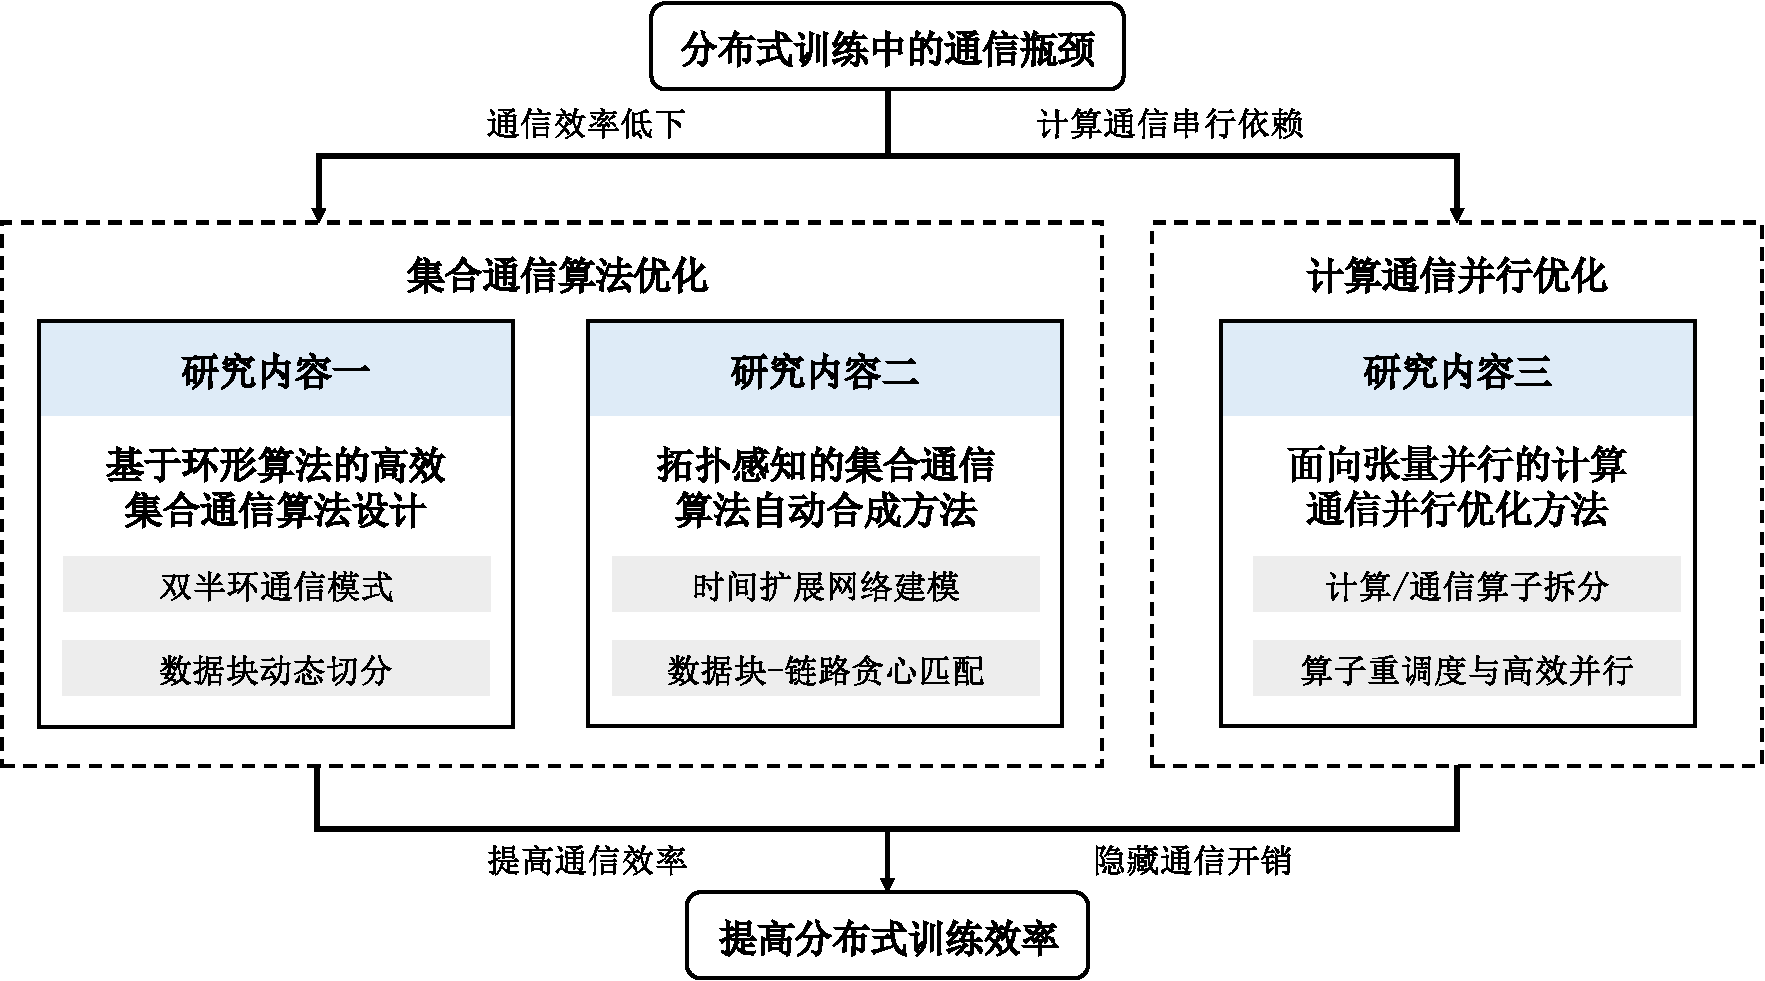
\includegraphics[width=\linewidth]{figure/chapter1/framework.pdf}
    \caption{\label{fig:framework}论文研究内容框架图}
\end{figure}

本文的主要创新点总结如下：
\begin{itemize}
  \item 由于分布式深度学习系统结构复杂，系统特征之间依赖性强，并且系统特征与训练时间之间呈现复杂的非线性关系，致使很难建立准确的训练时间预测模型。另外，现有的方法通常只能预测简单拓扑上的训练时间，如星形拓扑和环形拓扑。因此，本文提出了一种面向一般拓扑的分布式深度学习训练时间预测方法，首先对基于多层感知器（MLP）的计算时间预测模型引入额外的特征以提高预测精度，并通过分析深度学习框架中集合通信原语的执行机理和拓扑结构的通信特征建立细粒度的通信时间预测模型，最后基于计算与通信的并行关系分析建立了准确的训练时间预测模型。本文提出的预测方法适用于大部分拓扑上的分布式深度学习，比现有工作更具有通用性。
  \item 由于通信拓扑不仅决定了分布式训练每次迭代的通信开销，还影响着模型的收敛速度，现有的拓扑设计方法很难权衡二者得到高效的参数同步拓扑。因此，本文以一致性收敛速度为优化目标，以每次迭代的通信开销为约束条件，分别描述了同构带宽和异构带宽场景下的参数同步拓扑优化问题，并提出了基于ADMM算法和模拟退火算法的优化问题求解框架。通过求解优化问题得到的拓扑可以很好地权衡每次迭代的通信开销和一致性速度，提高分布式深度学习的训练效率。
  \item 考虑到现有的通信数据压缩方法的压缩误差会随着压缩程度的提高而增大，并且这些方法在带宽异构的场景下会导致资源浪费的问题，本文设计了带宽自适应的通信数据压缩方法，对基于压缩误差补偿的分布式随机梯度下降算法和分布式随机梯度跟踪算法引入带宽自适应策略，根据带宽矩阵调整每条边上通信数据的压缩程度，减小某些高带宽边上的数据压缩误差，提高模型精度和资源利用率。
\end{itemize}

\subsection{具体内容与章节安排}

本文各章节的研究内容安排概述如下：

第一章，绪论。本章首先介绍了分布式深度学习的发展概况并分析了训练时间预测与优化的必要性以及相应的研究挑战，然后针对国内外的研究现状进行了介绍，最后分析了现有方法存在的问题，提出了本文的研究思路与创新点，并对论文的章节安排进行了简要介绍。

第二章，面向一般拓扑的训练时间预测。本章首先分析了分布式深度学习训练时间预测的必要性与难点，引出了本章的研究内容。然后介绍了分布式训练时间的组成，并分析了影响计算时间的特征和影响通信时间的特征。接着基于特征分析结果设计了分布式深度学习训练时间预测方法，分别建立了计算时间预测模型和通信时间预测模型并进行了计算与通信的并行性分析以进一步提高预测精度。最后在真实GPU集群上测试分布式训练卷积神经网络模型所需的训练时间，进而分别对计算时间、通信时间和迭代时间预测结果进行了验证并对实验结果展开分析。

%引言部分可以介绍拓扑对每次迭代通信开销的影响和一致性速度的影响，然后介绍一致性在分布式深度学习的收敛性中起到的作用。
第三章，面向高效通信的参数同步拓扑优化。本章首先分析了参数同步拓扑对分布式深度学习训练时间的影响以及参数同步拓扑优化的难点，引出了本章的研究内容。其次介绍了典型线性平均一致问题，引出了拓扑优化问题的优化目标，并以每次迭代的通信开销为约束条件分别描述了同构带宽和异构带宽场景下的参数同步拓扑优化问题。然后，为了求解上述优化问题，提出了基于ADMM算法和模拟退火算法的优化问题求解框架，其中基于模拟退火算法生成的拓扑结构作为ADMM算法求解优化问题的初始条件，从而得到更好的求解结果。最后通过一致性实验以及基于Cifar10和Cifar100图像分类数据集的分布式训练实验验证了求解得到的拓扑的高效性，并对实验结果进行了分析。

第四章，带宽自适应的通信数据压缩。本章首先分析了通信数据压缩对分布式深度学习性能的影响以及现有的通信数据压缩方法存在的问题，引出了本章的研究内容。然后分别介绍了分布式深度学习中两种经典的基于去中心化架构的算法，分布式随机梯度下降（DSGD）算法和分布式随机梯度跟踪（DSGT）算法。接着，介绍了一种常用的量化策略以及相应的实现方式，并基于该量化策略和上述两种算法设计了相应的带宽自适应的量化分布式训练算法，设计的算法基于误差补偿降低量化误差，同时基于带宽矩阵调整每条边的压缩程度，进一步降低某些带宽较高的边上的数据压缩误差，提高模型精度。最后在Cifar10图像分类数据集上验证了所提出的量化分布式训练算法的有效性，并对实验结果进行了分析。

第五章，总结与展望。本章主要对本文的研究内容和创新点进行了简要的总结，对未来研究方向进行了展望。
